This is the page dedicated to describe and give general information about our association. It is formed by 4 main sections: 
\begin{itemize}
	\item \textbf{Who we are: } gives genral info about the association
	\item \textbf{Our Mission: } explains the purpose and final scope
	\item \textbf{History: } tells to user what the association as done from the foundation to today
\end{itemize}
A set of functional links has been added to let users easily navigate between these sections.

\subsubsection{About Us in-the-small}
\begin{figure}[h!]
	\centering
	\begin{minipage}[b]{1\textwidth}
    		
\includegraphics[width=\textwidth]{./assets/aboutus.png}
		\caption{About Us page - Design in the small}
	\end{minipage}
\end{figure}
\FloatBarrier

\clearpage

\subsubsection{About Us screenshot}
\begin{figure}[h!]
	\centering
	\begin{minipage}[b]{1\textwidth}
    		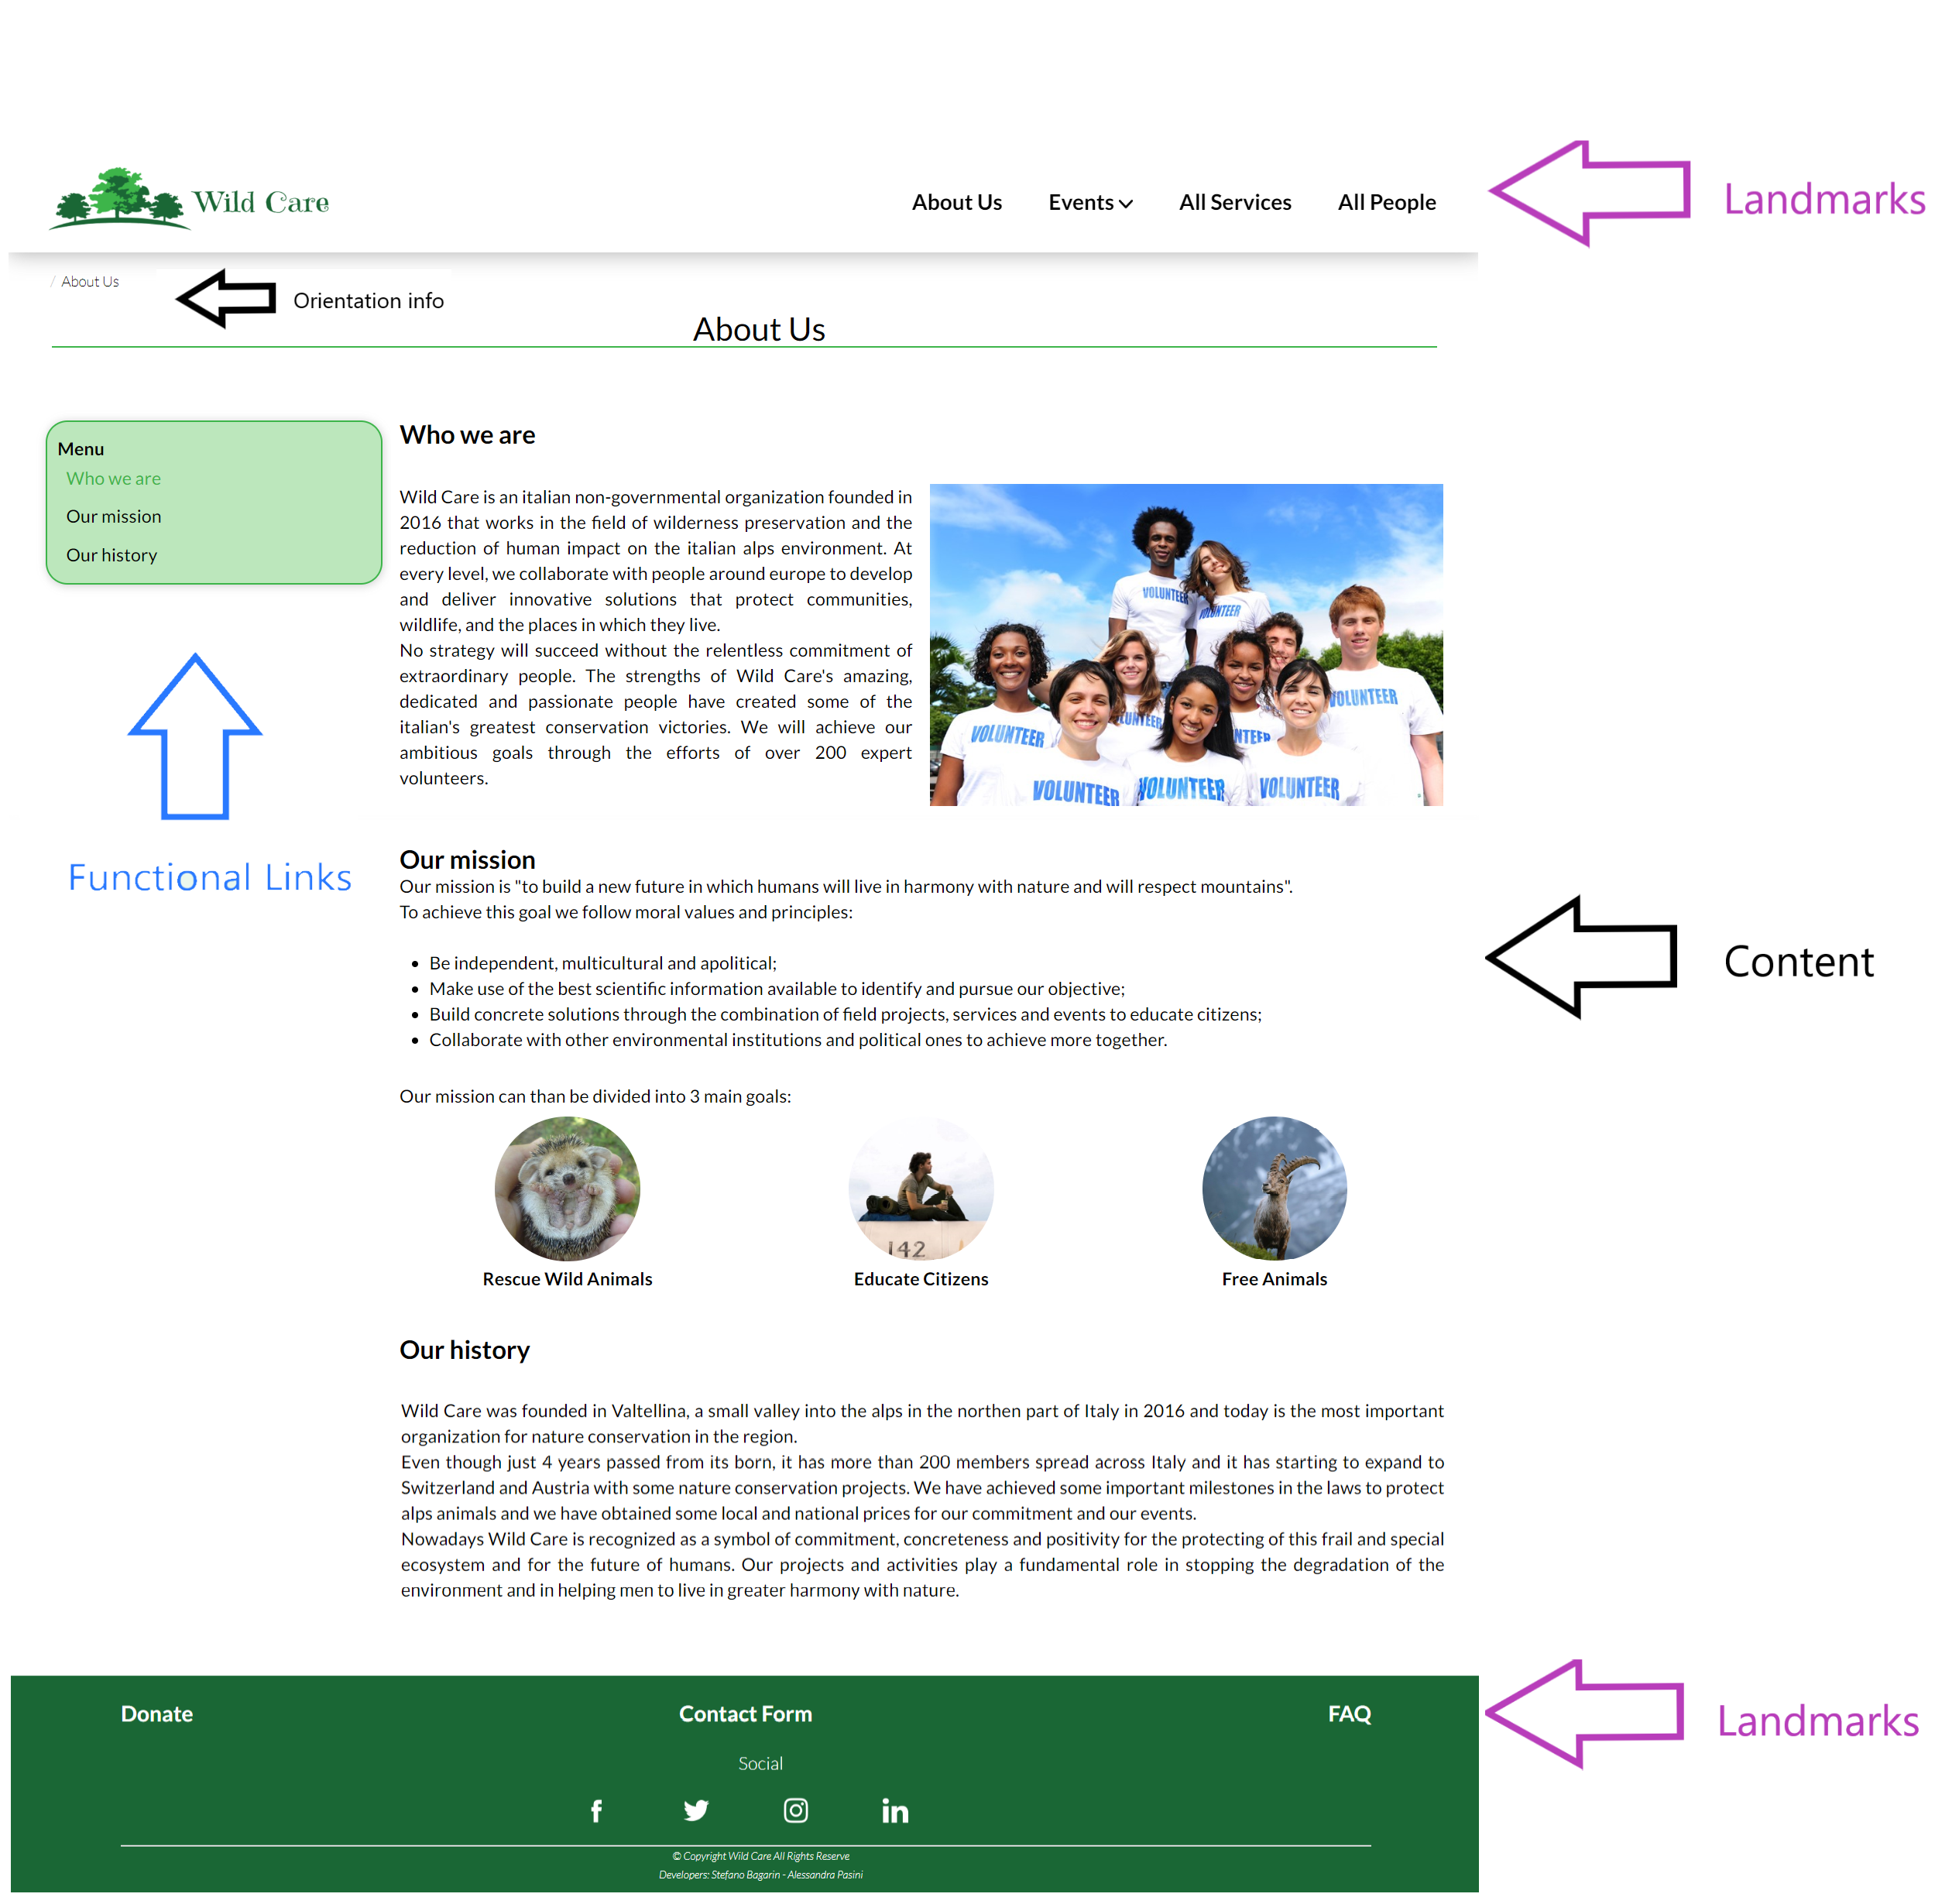
\includegraphics[width=\textwidth]{./assets/mockups/aboutus_commented.png}
		\caption{About Us page - Screenshot commented.}
	\end{minipage}
\end{figure}
\FloatBarrier

\clearpage


\subsection{Contact Form}
The aim of this page is to let users ask questions or send messages to the association through a contact form, whose fields are all mandatory. \\
Once filled the form, Send button must be clicked:
\begin{itemize}
	\item if one or more fields are empty or if the email is invalid (being valid means that it has the following structure: 				\emph{example@example.com}) an error message will occur;
	\item if the form has been well completed a success message will pop up.
\end{itemize}

\subsubsection{Contact Form in-the-small}
\begin{figure}[h!]
	\centering
	\begin{minipage}[b]{1\textwidth}
    		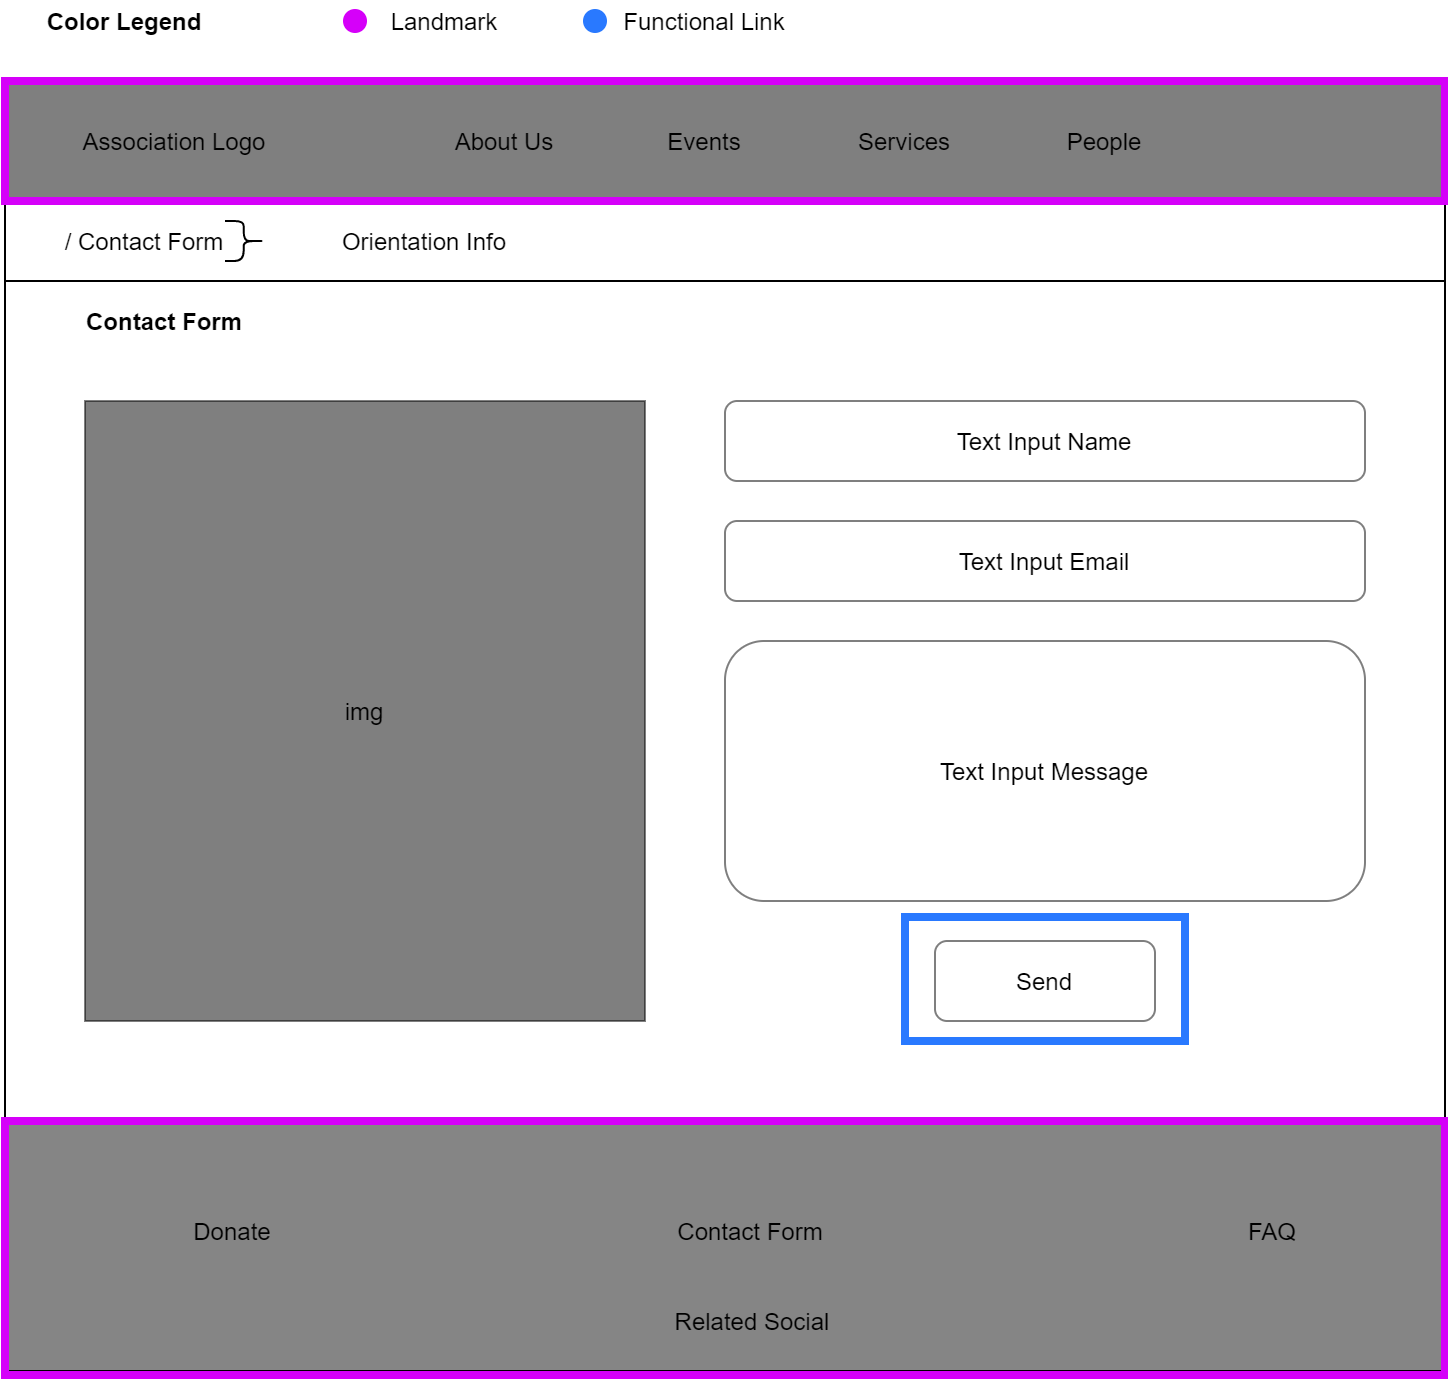
\includegraphics[width=\textwidth]{./assets/contactform.png}
		\caption{Contact Form page - Design in the small}
	\end{minipage}
\end{figure}
\FloatBarrier

\clearpage

\subsubsection{Contact Form screenshot}
\begin{figure}[h!]
	\centering
	\begin{minipage}[b]{1\textwidth}
    		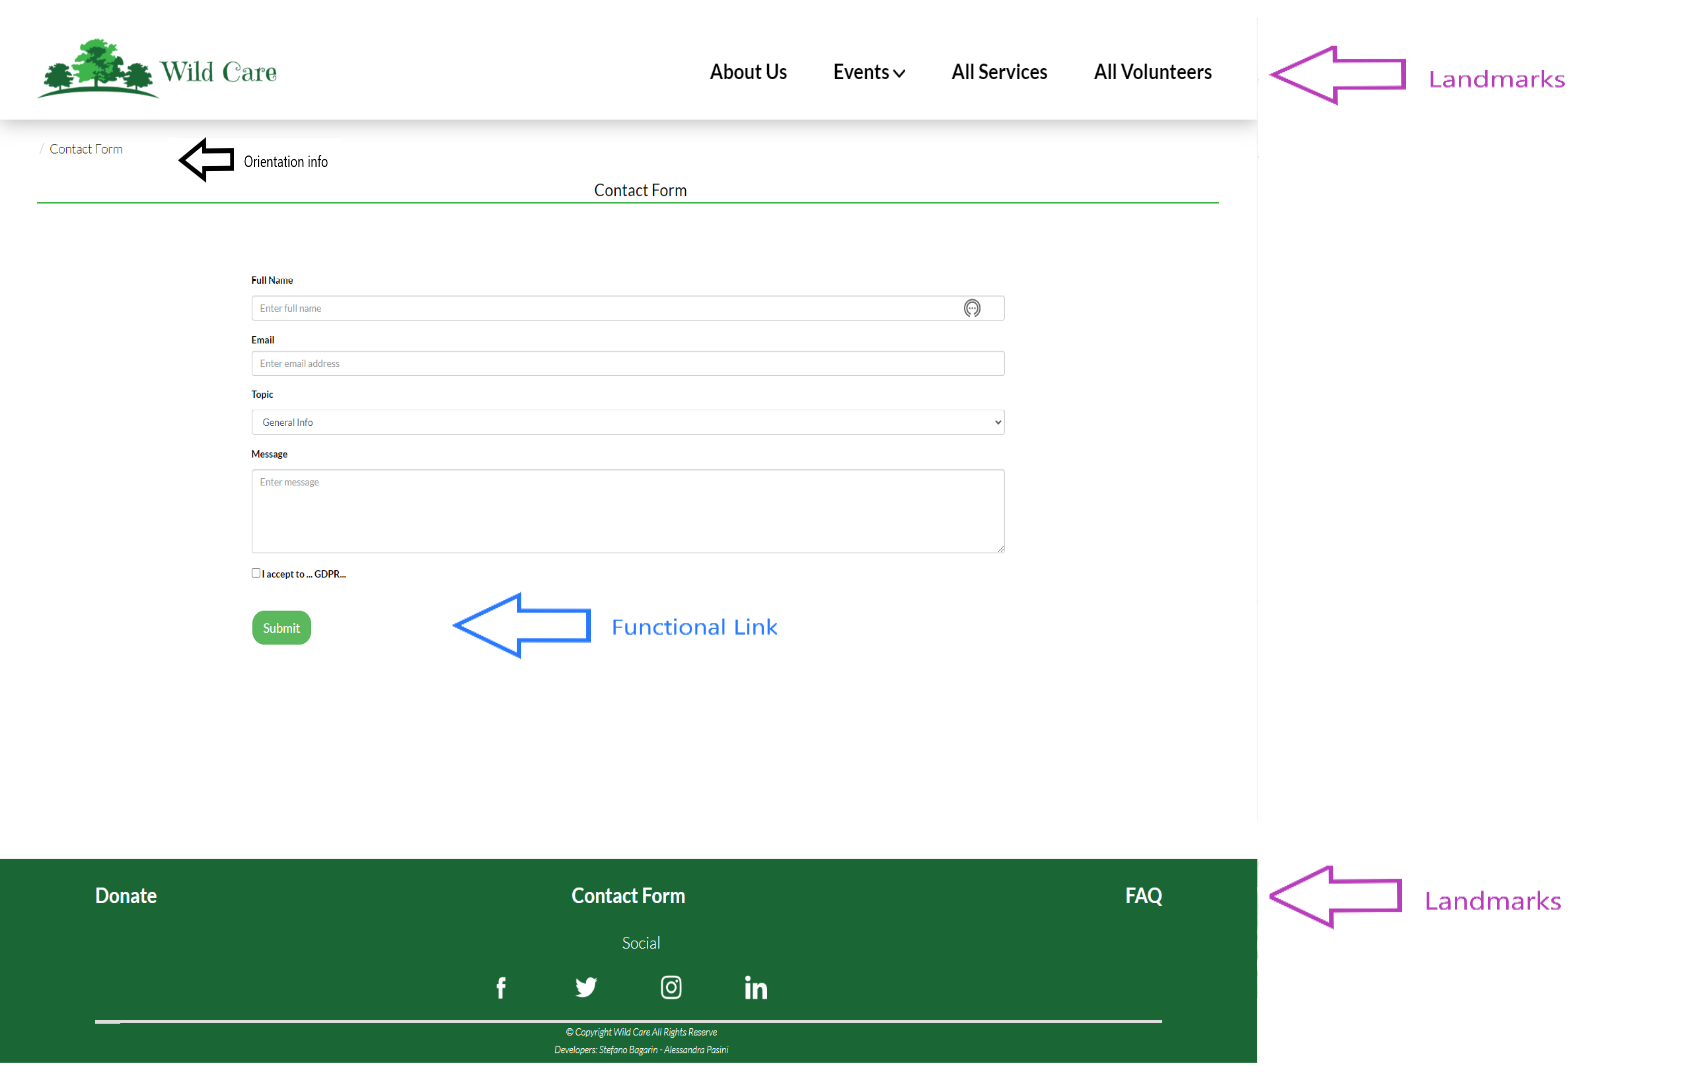
\includegraphics[width=\textwidth]{./assets/mockups/contactform_commented.png}
		\caption{Contact Form page - Screenshot commented.}
	\end{minipage}
\end{figure}
\FloatBarrier